The SE is a coarse-grained fabric composed of compute elements or tiles, which are interconnected with an SF, allowing data to traverse from one tile to another without queuing.
This SF allows many tiles to be pipelined together to produce a continuous data flow through SIMD arithmetic operations.
The tiles are also interconnected with an AF that allows synchronous domains of compute to be bridged by asynchronous operations.
These asynchronous operations include initiating SDF operations, transferring data from one SDF to another, accessing system memory (read and write), and performing branching and looping constructs.

\begin{figure} [h]
  \begin{subfigure}{.5\textwidth}
    \centering
    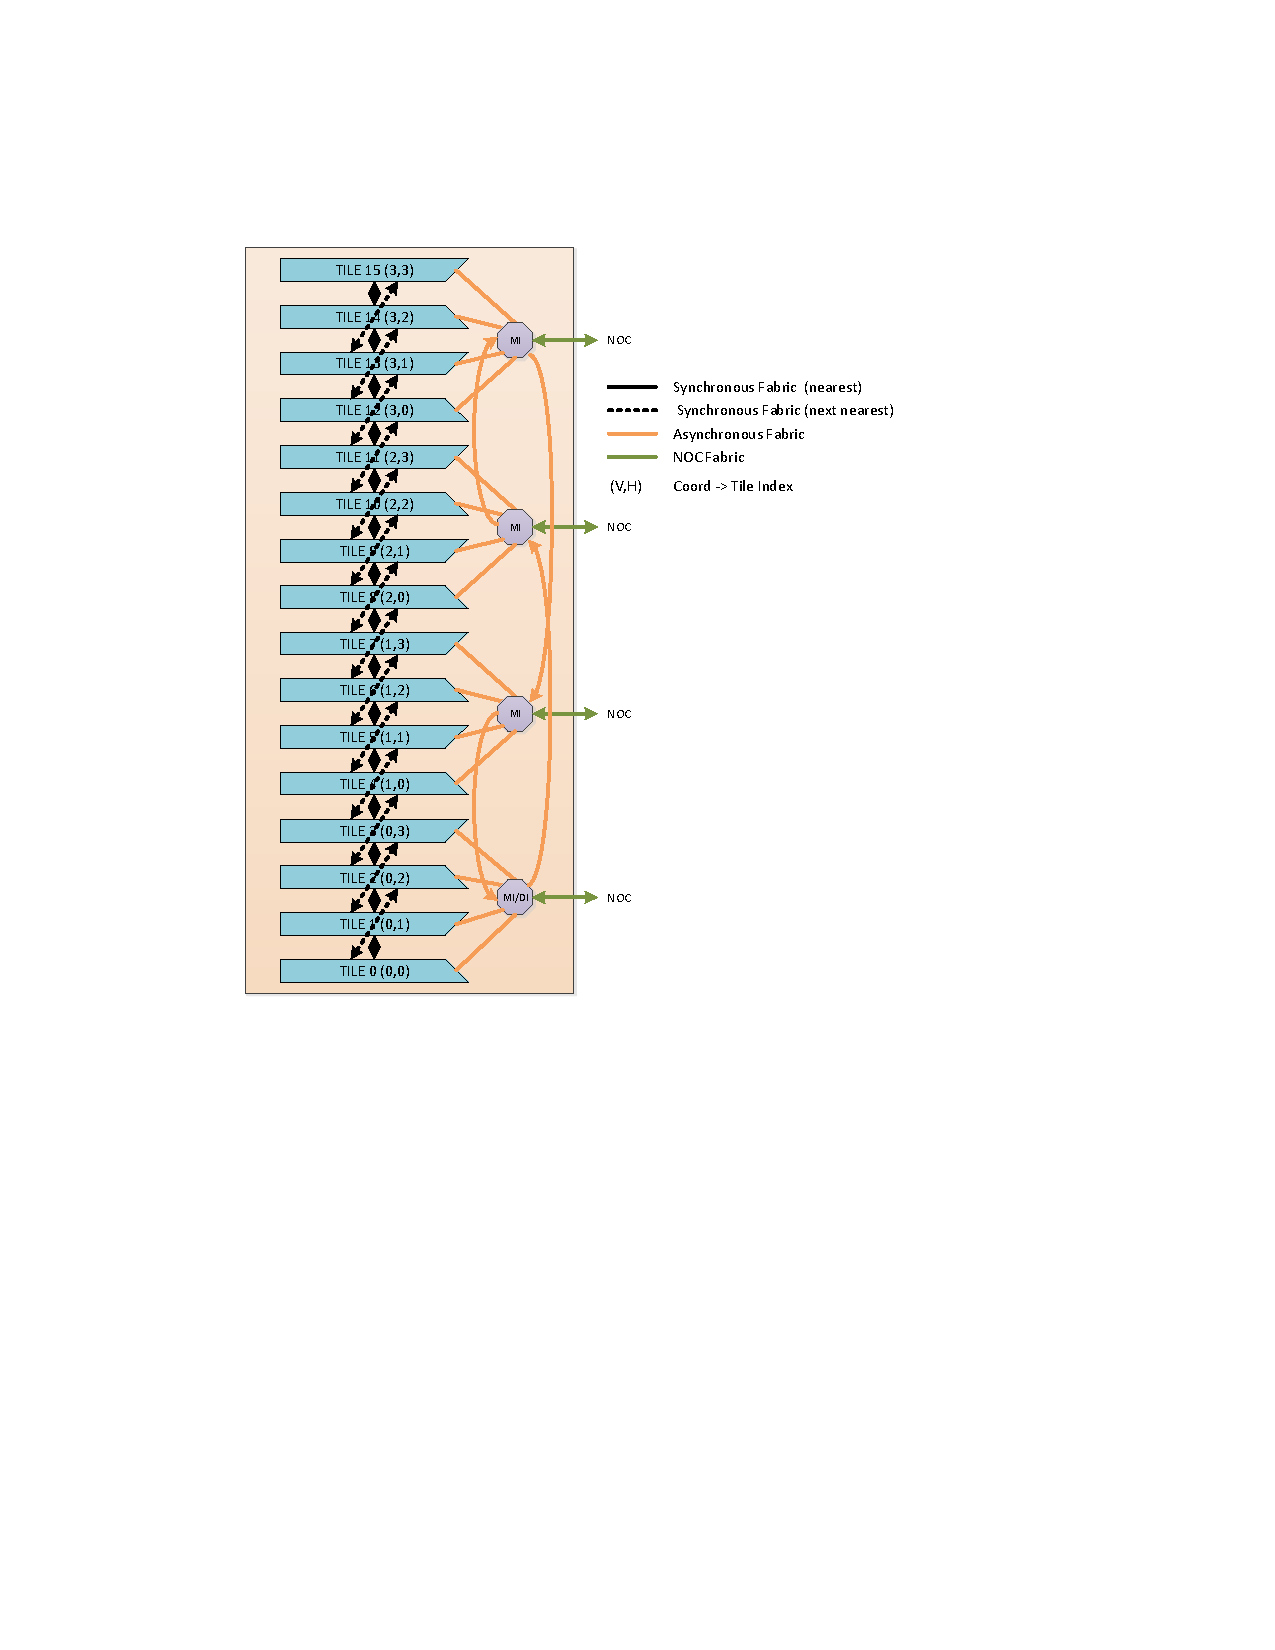
\includegraphics[trim=118 310 180 110, clip, width=0.7\linewidth]{fig/se_device.pdf}
    \caption{SE device}
    \label{fig:sub-se}
    \end{subfigure}
  \begin{subfigure}{.5\textwidth}
  \centering
  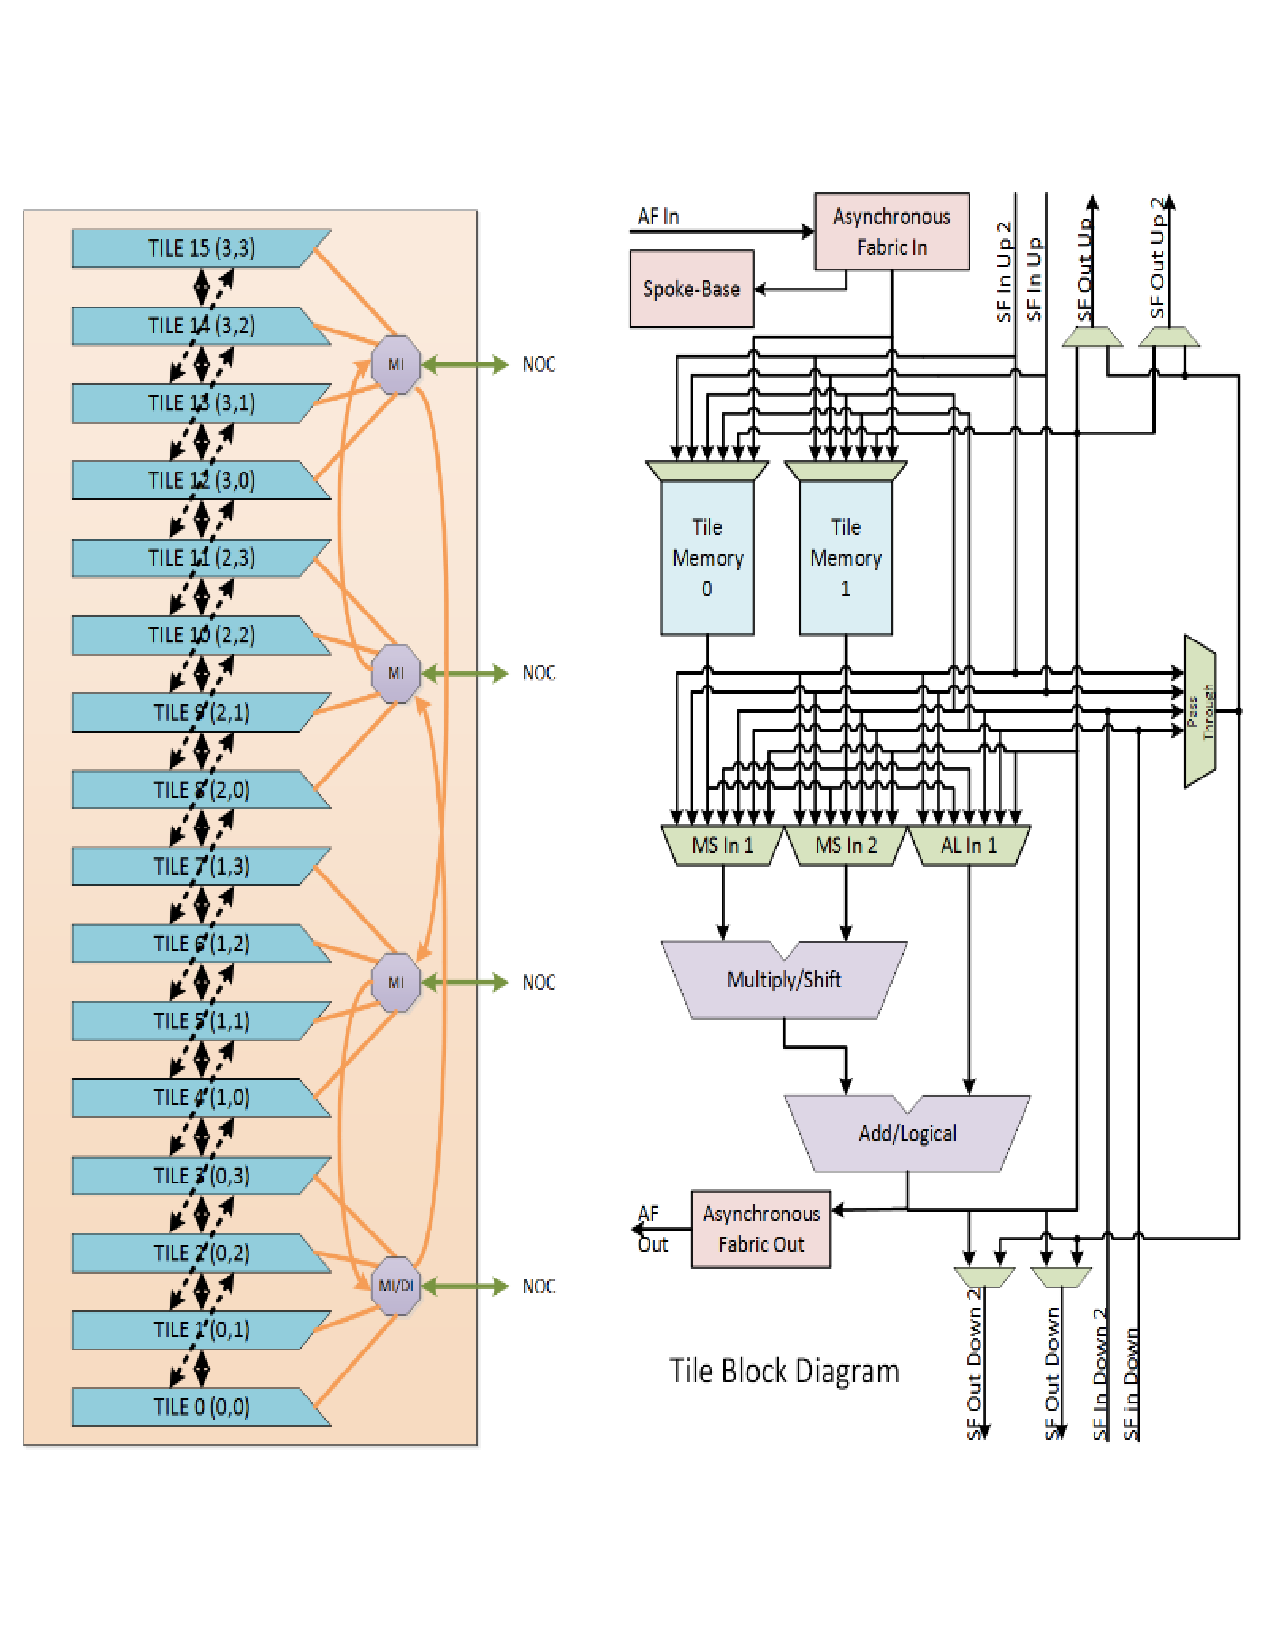
\includegraphics[trim=300 100 8 50, clip, width=0.5\linewidth]{fig/se_device_tile.pdf}
  \caption{SE tile}
  \label{fig:sub-tile}
  \end{subfigure}
  \caption{
    \figurename~\ref{fig:sub-se} shows layout of the SE device and dataflow paths between tiles. \figurename~\ref{fig:sub-tile} is a detailed diagram of a tile in the SE device. 
    Note the two tile memory units, the MS and AL units, and the four SF inputs and four SF outputs.
  }
  \label{fig:se_diagram}
\end{figure}

As shown in the \figurename~\ref{fig:se_diagram}, tiles are interconnected in a $1 \times 16$ configuration.
The SF is used to connect a tile to another tile one hop above it, a tile two hops above it, a tile one hop below it and a tile two hops below it.
Information is transferred over the SF with a deterministic latency. 
Each tile acts independently, streaming data through internal memory and MS/AL units to other tiles over the SF and AF.
The tiles use the AF to communicate between synchronous domains, send loads
 and stores to memory through the MI, and receive commands from the host through the DI to initiate work on the SE.
Information is transferred over the AF with a non-deterministic latency.


\subsection{Synchronous Fabric Interface}
All tiles that participate in a synchronous domain act as a single pipelined data path.
The Base Tile (BT) is defined as the first tile of a synchronous domain it initiates a thread of work through the pipelined tiles.
The BT is responsible for starting work on a predefined cadence, referred to as the Spoke Count or II.
E.g. For $II = 3$, as in the example in \figurename~\ref{fig:se_example}, then the BT can initiate work every third clock cycle.
%The synchronous fabric provides both data and control information.

\subsection{Asynchronous Fabric interface}
The Asynchronous Fabric is used to perform operations that occur asynchronously to a synchronous domain.
Each tile contains an interface to the AF.
AF messages can be classified as either data messages or control.
Data messages contain a SIMD width data value that is written to one of the two tile memories.
Control messages are for controlling thread creation, freeing resources, or issuing external memory requests.

\subsection{Tile Base}
The tile base contains data structures that are used to initiate an SDF.
%It receives messages from the SF interface to configure state and set up the necessary conditions to start a synchronous flow.
%It initiates a flow into the SF when the required conditions are met.
%It also contains control logic to manage iterations of loops.
A new thread is launched by the tile base of the BT every II.
The II allows the base logic to launch new threads or continue previously launched threads when all resources needed for execution are available.

\subsection{Tile Memory}
Each tile contains two memories.
Each are the width of the data path (512-bits), and the depth will be in the range of 512 to 1024 elements.
The tile memories are used to store data required to support data path operations.
The stored data can be constants loaded as part of the program's arguments, or variables calculated as part of the data flow.
The tile memory can be written from the AF as either a data transfer from another SDF, or the result of a load operation initiated by another SDF.
%The tile memory is only read via synchronous data path instruction execution.

\subsection{Instructions RAM}
Each tile has an instruction RAM has multiple entries to allow a tile to be time sliced, performing multiple, different operations in a pipelined synchronous domain.
%Additionally, each time slice could conditionally perform different instructions depending on previous tile time slice data dependent conditional operations. 

\subsection{Spoke RAM}
The Spoke RAM has multiple entries to reconfigure the tile at each time slice (clock cycle).
The number of active spoke RAM slots in a tile is equal to the II of that tile.
A couple of relevant configurations are: 

\begin{itemize}
  \item Which of the four SF inputs, feedback from the output of the tile's MS/AL unit, or the tile base is the master input.
  \item Which of the four SF outputs are used to send the output of the MS/AL unit to another tile or tiles using SF.
\end{itemize}

The Spoke RAM iterates over its slots using a counter that modulo counts from zero to II minus one and back to zero.
%Using different spoke counts on different tiles can be a powerful mechanism that allows the number of slices required by an inner loop to determine the performance of an application.
The proposed RL mapper provides the II and the configuration of each spoke RAM slot, including which tile instruction will be active, on each utilized tile.

\subsection{Programming the SE}
The SE programmer breaks down the desired application into a set of one or more SDFs.
An SDF is marked by instructions sending and receiving data in deterministic latency.
All operations with nondeterministic latencies, e.g. load/store requests to the MI, mark either the beginning and/or ending of an SDF.
We have a written an in-house parser that enables the programmer to express the program in terms of SDFs using our defined assembly language.
The parser produces an Intermediate Representation (IR) that is used as an input to our proposed mapper.

The IR represents each SDF as a graph, where every instruction a node.
Each node represents an instruction that needs to be placed onto a SE tile at the proper time-slice such that when all nodes are placed, the program executes correctly. 
In \figurename~\ref{fig:se_example}, the edges of the graph represent the data dependencies of the instructions. 
The nodes also contain information about the variables that need to be present in tile memories during instruction execution. 
The instruction intended to execute at a specific time-slice (clock cycle) will only execute when the master input configured in the corresponding Spoke RAM entry receives a valid control message.
%The tiles can pass data to their neighbors and each tile can be configured with a different number of initiation intervals (II). 
%Each II can be allocated to run a single instruction during program execution. 
%After one cycle, the tiles will move on to the next II, with execution returning to first II after the last. 
%All tiles run the instruction in the same II in parallel. 
%Thus, whenever possible, independent instructions should be mapped to different tiles and same II to exploit parallelism. 
%The first operation of each disconnected component of the computation graph (one component representing a synchronous flow) needs to be placed on different tiles. 

\subsection{SE Mapping Constraints}
The SE hardware imposes constraints that the RL mapper must adhere to in order to for it to produce a valid mapping. These constraints are:
\begin{enumerate}
  \item Instructions that share one or more tile memory variables must be placed on the same tile.
  \item No two or more instructions that start a synchronous data-flow can share a tile.
  \item No two or more instructions that are siblings in the SDF can share a tile.
\end{enumerate}
The SE device configuration and its constraints are modeled in a simulation environment and a reward function is used to determine the quality of placements obtained.
To enforce these constraints, we explore two methods in Section \ref{subsec:output_masking}.
The first method is to give a negative reward when a constraint is violated and the second is creation of a mask on the invalid actions so that the network only outputs valid actions.
In both cases, placing instructions sub-optimally leads to a reduced reward whereas placements that optimally reduce total execution time of the graph are rewarded. 